\section{Example with Gaussian hierarchical inference}
\label{sec: gaussian example}
\subsection{Without selection effects}
\label{subsec: example without selection effects}

We now consider a more concrete example with a simple hierarchical inference. To eliminate the effects of bias in the likelihood, we consider an example where there are no selection effects; all signals are detected. However, there is some noise associated with each signal, and this uncertainty must be marginalized over. In particular, our population draws events $\theta \sim \mathcal{N}(\mu, \sigma)$ from an underlying Gaussian population with mean $\mu$ and standard deviation $\sigma$. We note these simulation studies are very similar to those in Sec. III in \citet{Essick:2022ojx}.

Suppose there is some noise $n\sim\mathcal{N}(0, \sigma_n)$ where we observe $d=\theta+n$. Then, we have a Gaussian likelihood for each event
\beq
p(d|\theta) = \frac{1}{\sqrt{2\pi\sigma_n^2}}\exp\left(-\frac{(d-\theta)^2}{2\sigma_n^2}\right)
\eeq
For a collection of events $\{d_i\}$, we can compute the hierarchical likelihood of Eq.~\ref{eq: rate marginalized likelihood} in closed form (ie. we have a ``ground truth'' for comparison), and also estimate using the traditional Monte Carlo approach of Eq.~\ref{eq: estimated hierarchical likelihood}
\begin{align}
\mathcal{L}(\{d_i\}|\Lambda) &= \prod_{i=1}^{\Nobs} \int p(d_i|\theta)p(\theta|\Lambda)\dd\theta = [2\pi(\sigma^2 + \sigma_n^2)]^{-N_{\rm obs} / 2}\exp\left[-\sum_{j=1}^{N_{\rm obs}}\frac{(d_j - \mu)^2}{2(\sigma^2 + \sigma_n^2)}\right] 
\label{eq: analytic gaussian likelihood} \\
\hat{\mathcal{L}}(\{d_i\}|\Lambda) &= \prod_{i=1}^{\Nobs}\hat{p}(d_i|\Lambda),
\qquad\qquad{\rm where}\qquad\qquad
\hat{p}(d_i|\Lambda)=\left[\frac{1}{\NPE}\sum_{j=1}^{\NPE}\frac{p(\theta_{ij}|\Lambda)}{\pi(\theta_{ij}|{\rm PE})}\right]_{\theta_{ij} \sim p(\theta|d_i)}.
\label{eq: estimated gaussian likelihood}
\end{align}
For all the single event \ac{PE}, we use an improper uniform prior $\pi(\theta|{\rm PE})\propto 1$, so drawing $\theta_j$ from the posterior $p(\theta|d_i)$ is drawing from a Gaussian with mean $d_i$ and standard deviation $\sigma_n$. 

We calculate the posterior on the population hyperparameters $\mu, \sigma$ with a uniform hyperprior $\pi(\mu)=U(0,2)$ and $\pi(\log_{10}\sigma) = U(-1,1)$.
Though the likelihood estimator is unbiased, we know from Section~\ref{sec: bias in population inference} that the resulting posteriors will be biased. In addition, there is uncertainty in the posterior estimators, and we quantify the uncertainty and bias with the precision and accuracy statistics of Eqs.~\ref{eq: precision statistic} and \ref{eq: accuracy statistic}. To compute these statistics we need
\beq
\hat{C}_{\ln\mathcal{L}}(\Lambda, \Lambda') =  \sum_{i=1}^{\Nobs}\frac{\hat{C}_{p_i}(\Lambda, \Lambda')}{\hat{p}(d_i|\Lambda)\hat{p}(d_i|\Lambda')},
\label{eq: gaussian example covariance}
\eeq
which is the estimator for the covariance in the log-likelihood of two hyperparameter points $\Lambda$ and $\Lambda'$. 

\begin{figure}
    \centering
    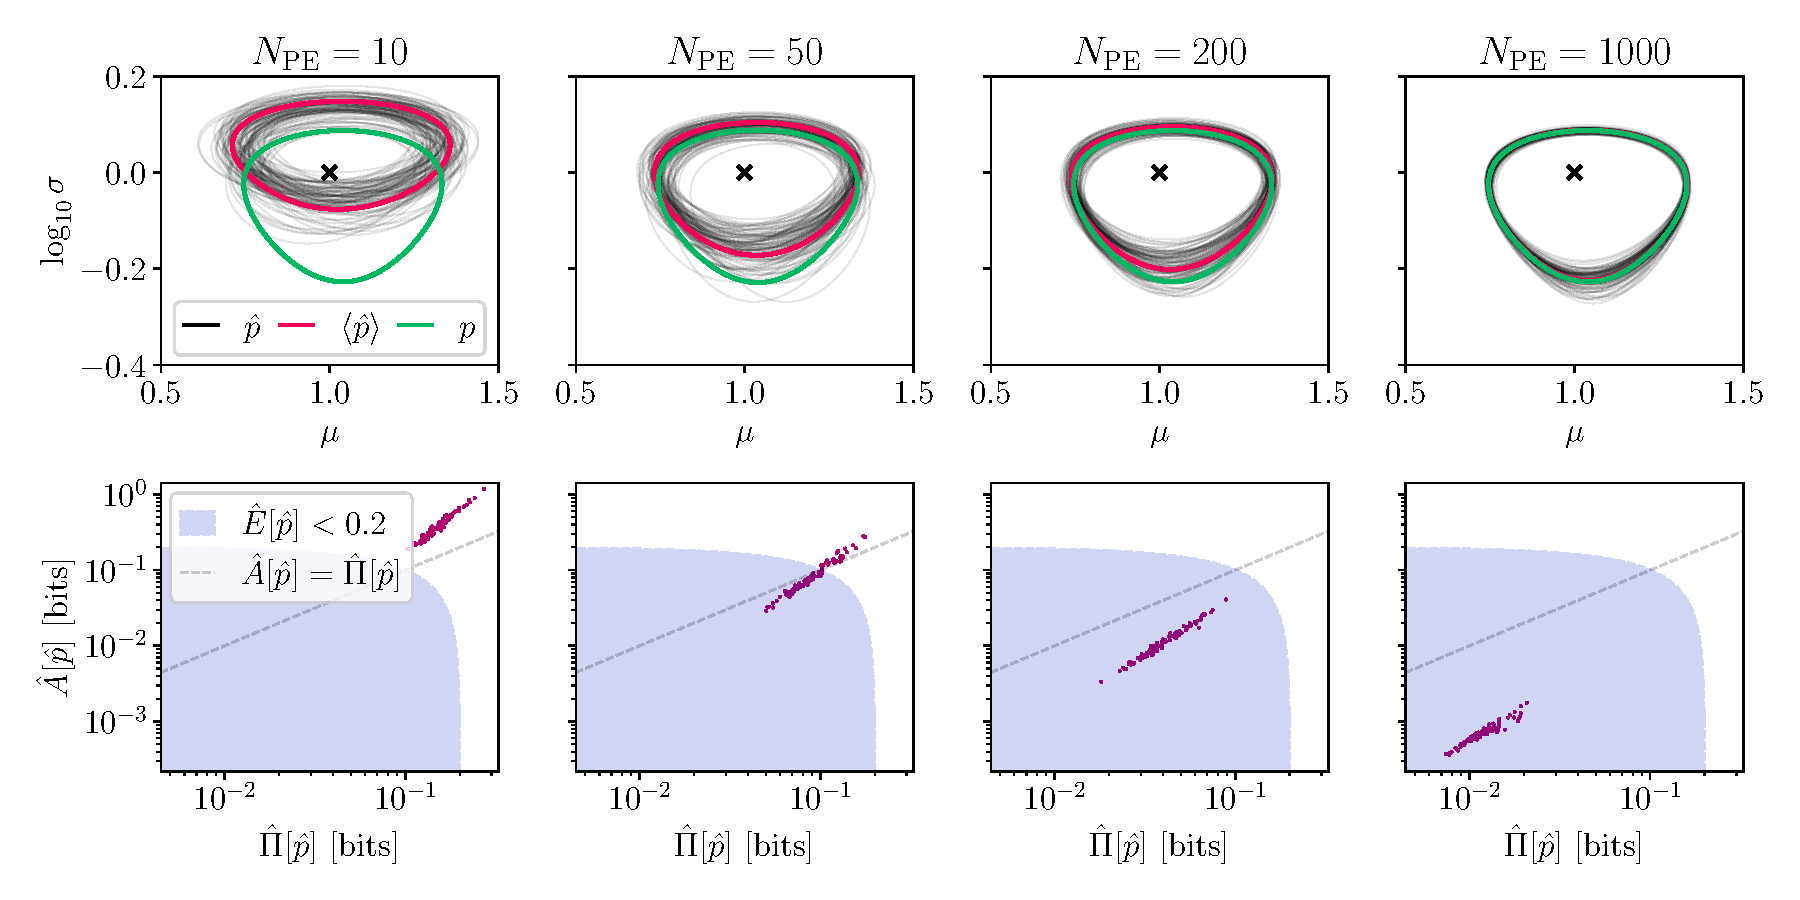
\includegraphics[width=\linewidth]{plots/gaus_hierarchical/pe_uncertainty_only/N100_4pes_scatter.pdf}
    \caption{Inference in a Gaussian hierarchical inference with 100 observations and a variable number of \ac{PE} samples. Here, the scale of the noise is comparable to the size of the population ($\sigma_n=\sigma=1$). In the upper panels, we show the 90\% \HPD contours of the Monte Carlo posterior estimators $\hat{p}$ (black) compared to the true posterior $p$ (green) and the mean of the posterior estimators $\langle\hat{p}\rangle$. We show the true value of the population hyperparameters with a black $\times$ symbol ($\mu=1$ and $\sigma = 1$). In the lower panels, we show the accuracy and precision statistics for each posterior estimator and the threshold for a reliable posterior estimator $\hat{E}[\hat{p}] < 0.2$ bits.}
    \label{fig: nobs 100 gaussian example}
\end{figure}

In this simplified setting, where the hyperposterior is only two dimensional, we can directly compute the analytic posterior density (with Eq.~\ref{eq: analytic gaussian likelihood}) over a grid of appropriate $\mu$, $\sigma$ values, the Monte Carlo estimator of the posterior density, and the accuracy and precision statistics (using Eqs.~\ref{eq: precision statistic},~\ref{eq: accuracy statistic} and \ref{eq: gaussian example covariance}). In Fig.~\ref{fig: nobs 100 gaussian example}, we show a comparison between the Monte Carlo posterior estimates (in black), the average of the Monte Carlo posteriors (red), and the true analytic posterior (green). Each Monte Carlo posterior estimate has a different randomized set of samples drawn from the single-event posteriors. In the upper panels, the Monte Carlo posterior estimators compared to the true posterior and the mean of the posterior estimators. The lower panels show the precision and accuracy statistics for each posterior estimator. As the number $\NPE$ of \PE samples increases for each Monte Carlo integral, the bias begins to disappear below noise between the different posterior estimators -- the accuracy statistic decreases below the precision statistic. Fig.~\ref{fig: nobs 100 gaussian example} is for an example with $\Nobs=100$ observations.

We showed in Section~\ref{sec: robustness measures} that thresholding on the variance in the log-likelihood estimator is enough to bound the total error statistic. However sometimes it is much stronger than necessary, especially for simple population models (like the Gaussian population model we use here) with a large number of observations. In the bottom row of Fig.~\ref{fig: nobs 5000 ehat vs var}, we compare the error statistics to the mean log-likelihood variance across the posterior when using $\Nobs = 5000$ observations. We show that the error statistic can be very small even when the variance in the log-likelihood is large --- see the furthest right panels, using $\NPE = 1000$. The posterior estimators are clearly strongly clustered on the correct posterior (upper panel) and the error statistics correctly reflect this: $\hat{E}[\hat{p}] \sim 0.03$ bits, while the variance is quite large, $\hat{\sigma}^2 \sim 5$.

We show further examples with $\Nobs = 1000$ and $\Nobs = 5000$ and a comparison where the population structure $\sigma$ is smaller than the noise in each single event $\sigma_n$ in the Appendix~\ref{app: gaussian pe uncertainty only}. 

\begin{figure}
    \centering
    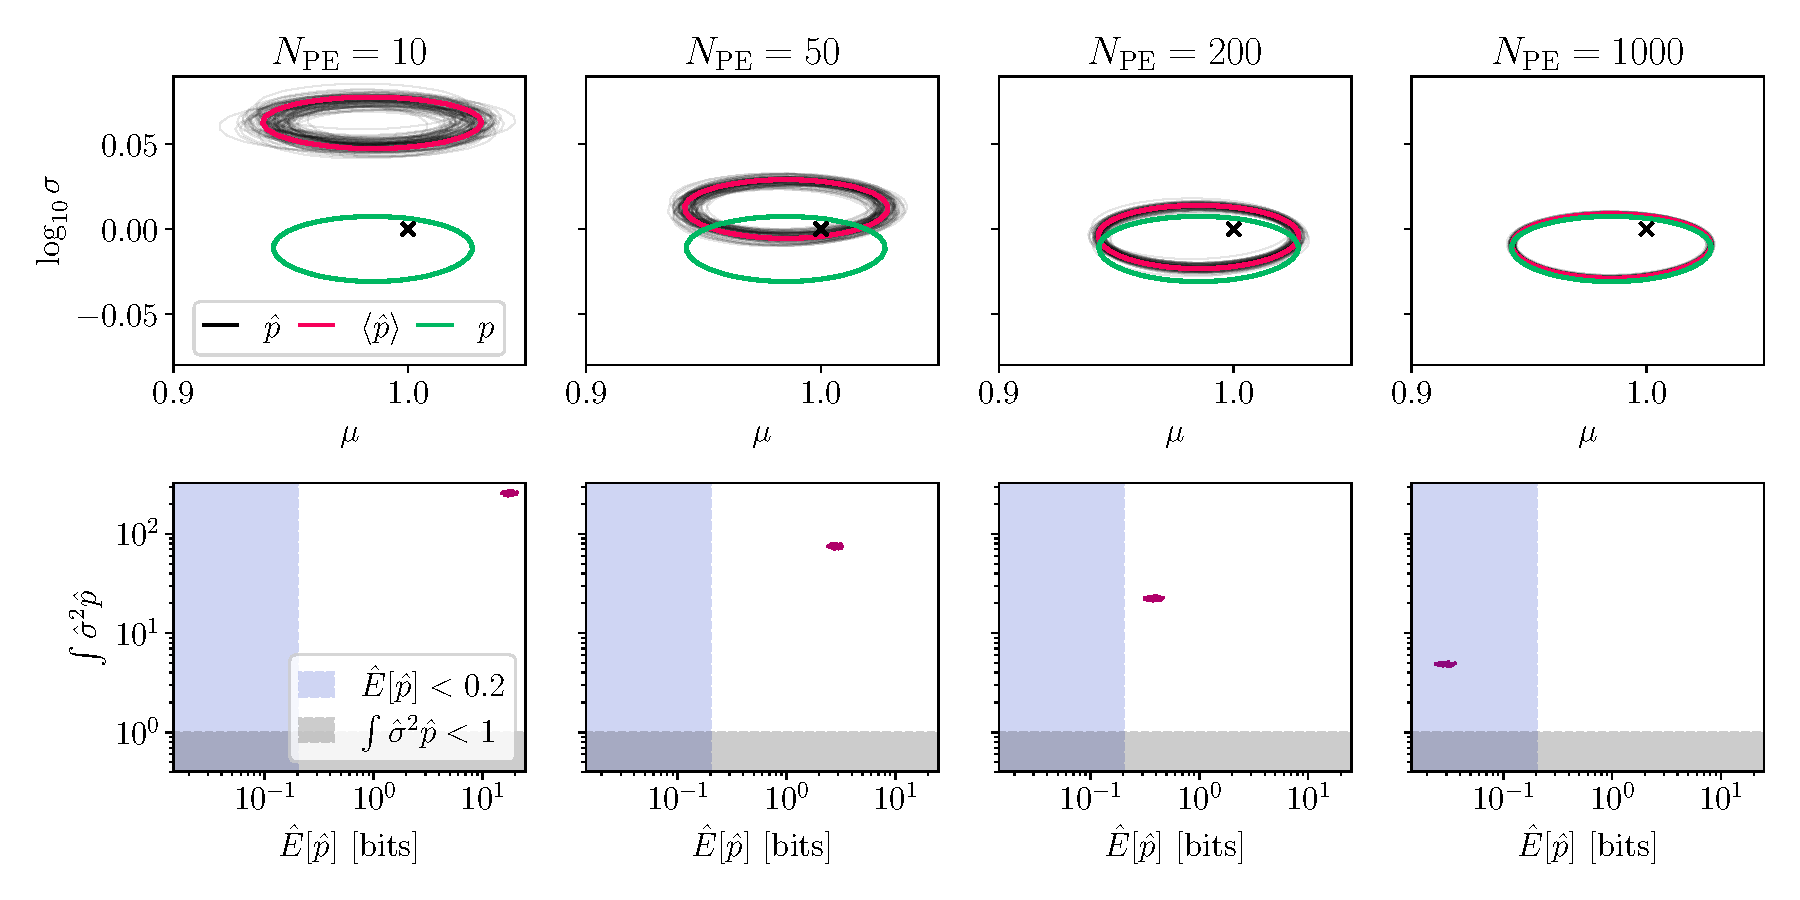
\includegraphics[width=\linewidth]{plots/gaus_hierarchical/pe_uncertainty_only/N5000_4pes_scatter_error_vs_var.pdf}
    \caption{Analogous to Fig.~\ref{fig: nobs 100 gaussian example} with $\Nobs = 5000$. In the bottom row, we compare the mean variance estimator across the posterior ($\int \hat{\sigma}^2\hat{p}$) to the error statistic for each posterior estimator and demonstrate that the error in a posterior estimator is more accurately described by the error statistic than the variance in the log-likelihood estimator.}
    \label{fig: nobs 5000 ehat vs var}
\end{figure}

\begin{figure}[h!]
    \centering
    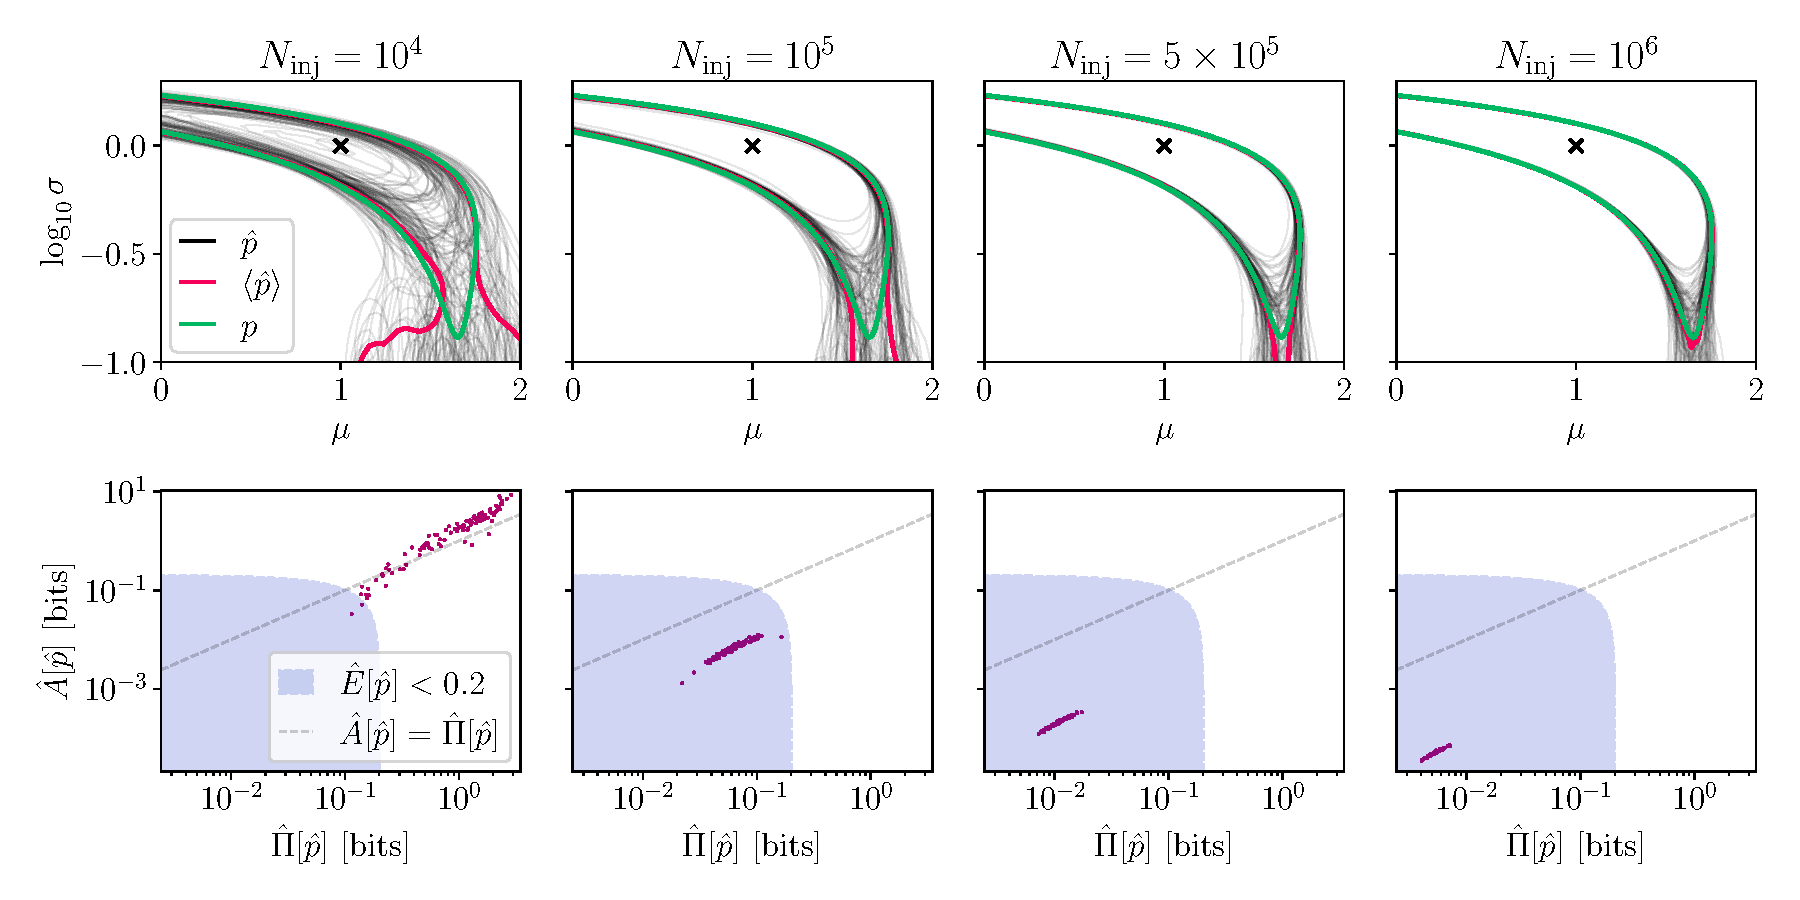
\includegraphics[width=\linewidth]{plots/gaus_hierarchical/selection_effects/selection_1_N100_4vts_scatter_noLikelihoodCorrection.pdf}
    \caption{Analogous to Fig.~\ref{fig: nobs 100 gaussian example} where we select events for detection using $d=\theta+n > \thresh$ where $\thresh = 1$. We estimate the likelihood using Eq.~\ref{eq: estimated gaussian likelihood with vt}. We use $\Nobs=100$ observations and compare $\Ninj = 10^4,10^5,5\times10^5$ and $10^6$.}
    \label{fig: nobs 100 vt 1 gaussian example}
\end{figure}

\subsection{Example with selection effects}
\label{subsec: example with selection effects}

As another example, we consider a similar example as the above, where events are drawn from an underlying Gaussian population $\theta \sim\mathcal{N}(\mu, \sigma)$ and we observe data $d=\theta+n$ obscured by noise $n\sim\mathcal{N}(0,\sigma_n)$. This time, however, we include a selection effect where we only detect events such that $d > \thresh$ exceeds the threshold $\thresh$. We again note these simulation studies are very similar to those in Sec. III in \citet{Essick:2022ojx}.

We may still compute the hierarchical likelihood of Eq.~\ref{eq: rate marginalized likelihood} in closed form (ground truth)
\beq
\mathcal{L}(\{d_i\}|\Lambda) = \left[\frac{1}{2}{\rm erfc}\left(\frac{\thresh-\mu}{\sqrt{2(\sigma^2+\sigma_n^2)}}\right)\right]^{-\Nobs}[2\pi(\sigma^2 + \sigma_n^2)]^{-N_{\rm obs} / 2}\exp\left[-\sum_{j=1}^{N_{\rm obs}}\frac{(d_j - \mu)^2}{2(\sigma^2 + \sigma_n^2)}\right],
\label{eq: analytic gaussian likelihood with vt}
\eeq
which is identical to Eq.~\ref{eq: analytic gaussian likelihood} but now includes an analytic selection effects term $\alpha(\Lambda)^{-\Nobs}$ using the complementary error function erfc.

We also compute a variant of the hierarchical likelihood where we calculate the single-event integrals analytically but we estimate the selection effects term with a Monte Carlo integral
\beq
\hat{\mathcal{L}}(\{d_i\}|\Lambda) = \left[\frac{1}{\Ninj}\sum_{j=1}^{\Nfound}\frac{p(\theta_{i}|\Lambda)}{p(\theta_{i}|{\rm draw})}\right]_{\theta_{i} \sim p(\theta|{\rm draw})}^{-\Nobs}[2\pi(\sigma^2 + \sigma_n^2)]^{-N_{\rm obs} / 2}\exp\left[-\sum_{j=1}^{N_{\rm obs}}\frac{(d_j - \mu)^2}{2(\sigma^2 + \sigma_n^2)}\right].
\label{eq: estimated gaussian likelihood with vt}
\eeq
We can also think of this as the traditional estimator of Eq.~\ref{eq: estimated hierarchical likelihood} when we take the limit $\NPE \to \infty$. We take the draw distribution for estimating selection effects to be $p(\theta|{\rm draw}) = \mathcal{N}(\mu_{\rm vt}=1,\sigma_{\rm vt}=1.5)$.\footnote{Using Eq.~\ref{eq: variance of Monte Carlo integral}, one can show that the Monte Carlo estimator for the selection effects has a infinite variance when $\sigma^2 > 2\sigma_{\rm vt}^2$, and so the estimator is always unreliable for $\sigma \gtrsim 2.12$. We restrict the hyperprior on $\log_{10}\sigma$ to avoid this domain. In practice, the correction term in Eq.~\ref{eq: unbiased likelihood estimator} should also strongly downweight this region.}

We assume uniform hyperpriors $\pi(\mu)=U(0,2)$ and $\pi(\log_{10}\sigma) = U(-1,0.3)$.
We show a comparison between the posterior estimators, the mean of the posterior estimators, and the true posterior in Fig.~\ref{fig: nobs 100 vt 1 gaussian example} where $\Nobs=100$ observations and the selection given by $\thresh = 1$. In the lower panels we show the accuracy and precision statistics for each posterior estimator compared to the region $\hat{E}[\hat{p}] < 0.2$ bits.
The accuracy and precision statistics (Eqs.~\ref{eq: precision statistic} and \ref{eq: accuracy statistic}) rely on the covariance estimator, which for this problem is given as the \textit{second} term in Eq.~\ref{eq: population covariance with selection},
\beq
\hat{C}_{\ln\mathcal{L}}(\Lambda, \Lambda') = \frac{\Nobs^2\hat{C}_{\xi}(\Lambda, \Lambda')}{\hat{\xi}(\Lambda)\hat{\xi}(\Lambda')}.
\label{eq: vt gaussian example covariance}    
\eeq

Moving to the right in Fig.~\ref{fig: nobs 100 vt 1 gaussian example}, we increase the size $\Ninj$ of the Monte Carlo integrals. Notice the error statistics drop below the recommended threshold, and the error becomes dominated by the precision statistic (the points in the lower panel move below the diagonal dashed line).

For small $\Ninj$, the likelihood estimator in Eq.~\ref{eq: estimated gaussian likelihood with vt} is significantly biased. When we include the likelihood correction term of Eq.~\ref{eq: unbiased likelihood estimator}, this alters the posterior estimators and shifts them away from the biased regime (small $\log_{10}\sigma$); see Fig.~\ref{fig: nobs 100 corrected vt 1 gaussian example}. There is still bias in the posterior, which we discuss in greater detail in Appendix~\ref{app: additional gaussians}.
\begin{figure}
    \centering
    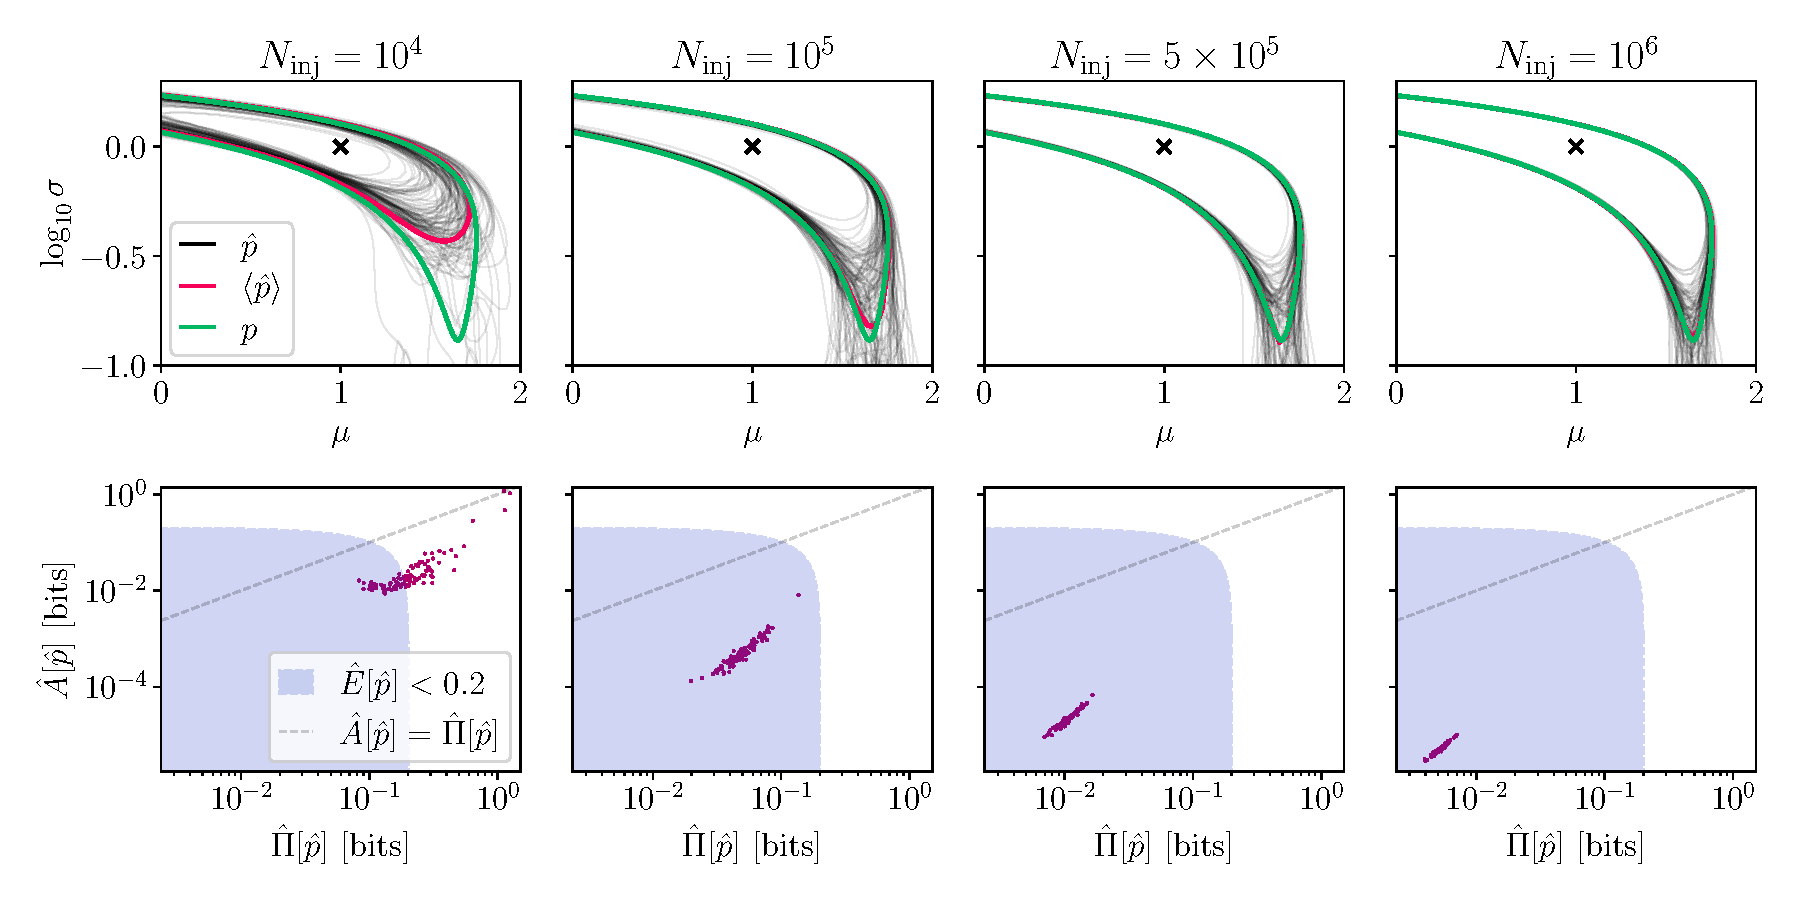
\includegraphics[width=\linewidth]{plots/gaus_hierarchical/selection_effects/selection_1_N100_4vts_scatter.pdf}
    \caption{Analogous to Fig.~\ref{fig: nobs 100 vt 1 gaussian example} using the corrected likelihood estimator of Eq.~\ref{eq: unbiased likelihood estimator}. Notice, particularly for small $\Ninj$, the improved behavior of the mean posterior estimator $\langle\hat{p}\rangle$.}
    \label{fig: nobs 100 corrected vt 1 gaussian example}
\end{figure}


\subsection{Asymptotic scaling and verification}

\begin{figure}[h!]
    \centering
    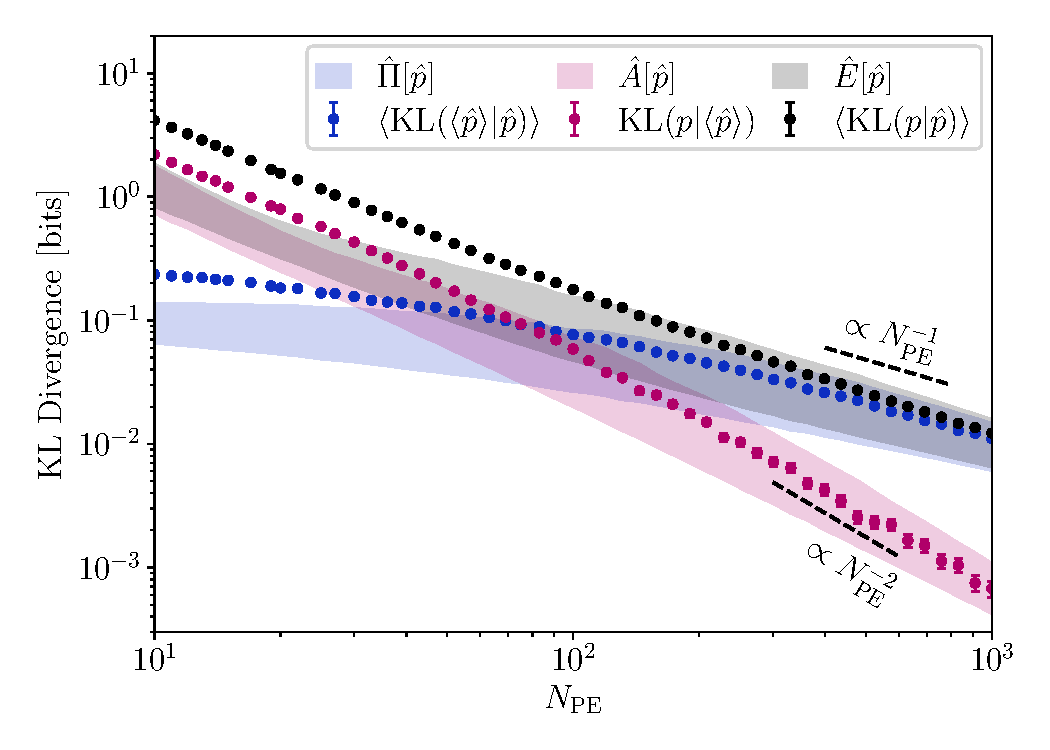
\includegraphics[width=0.6\linewidth]{plots/expKL_npe_vs_est.pdf}
    \caption{A comparison between the empirically measured \KL divergences (using $10^4$ posterior estimators) and their corresponding estimators, as a function of $\NPE$. We use the simple Gaussian hierarchical inference problem of Section~\ref{subsec: example without selection effects} with $\Nobs = 100$ where the prior for the mean is fixed to the true value $\pi(\mu) = \delta(\mu-1)$. In blue, we show the empirically measured average \KL divergence from the mean of the posterior estimators $\langle\KLD(\langle\hat{p}\rangle|\hat{p})\rangle$. For each posterior estimator, this \KL divergence is itself estimated by the precision statistic $\hat{\Pi}[\hat{p}]$. We show the central 90\% interval for the precision statistic in the blue shaded region, and show that $\langle\KLD(\langle\hat{p}\rangle|\hat{p})\rangle$ and $\hat{\Pi}[\hat{p}]$ asymptotically scale as $\NPE^{-1}$. Similarly, in red we show the empirically measured \KL divergence from the true posterior to the mean of the posterior estimators $\KLD(p|\langle\hat{p}\rangle)$. This is estimated by the accuracy statistic $\hat{A}[\hat{p}]$; the 90\% interval of $\hat{A}[\hat{p}]$ is shaded in red. These quantities, $\KLD(p|\langle\hat{p}\rangle)$ and $\hat{A}[\hat{p}]$ asymptotically scale as $\NPE^{-2}$. Finally, the black points show the empirically measured mean \KL divergence from the true posterior to a posterior estimator $\langle\KLD(p|\hat{p})\rangle$. To leading order, we estimate this with the error statistic $\hat{E}[\hat{p}] = \hat{\Pi}[\hat{p}] + \hat{A}[\hat{p}]$, shaded in black. At large values of $\NPE$, the precision statistic is the dominant contribution to the error and so the error scales as $\NPE^{-1}$. At small values of $\NPE$, higher order terms in the \KL divergence contribute and so the statistics tend to underestimate to the \KL divergences. As $\NPE$ increases, the precision, accuracy and error statistics begin to center on their correct, empirically measured values.} 
    \label{fig: random KL fn of npe}
\end{figure}

We show here that the precision, accuracy and error statistics are valid estimators for the information-loss they are meant to quantify. The precision statistic $\hat{\Pi}[\hat{p}]$ estimates the average information loss in the posterior estimator due to random scatter. Formally, it estimates the average \KL divergence from the \textit{mean} of the posterior estimators $\langle\KLD(\langle\hat{p}\rangle|\hat{p})\rangle$. The accuracy statistic $\hat{A}[\hat{p}]$ estimates the information lost due to bias in the posterior estimators; the \KL divergence from the true posterior to the mean of the posterior estimators $\KLD(p|\langle\hat{p}\rangle)$. The error statistic, which we calculate as the sum of the accuracy and precision statistics $\hat{E}[\hat{p}] = \hat{\Pi}[\hat{p}] + \hat{A}[\hat{p}]$, estimates the leading order average \KL divergence from the true posterior $\langle\KLD(p|\hat{p})\rangle$. 

We use the simple Gaussian hierarchical inference model introduced above in Section~\ref{subsec: example without selection effects} to empirically calculate the \KL divergences $\langle\KLD(\langle\hat{p}\rangle|\hat{p})\rangle$, $\KLD(p|\langle\hat{p}\rangle)$ and $\langle\KLD(p|\hat{p})\rangle$ from an ensemble of $10^4$ posterior estimators. 
We show that the precision statistic, accuracy statistic and error statistics all reliably estimate the associated \KL divergences at larger values of $\NPE$. 
At small values of $\NPE$ (large uncertainties in the log-likelihood estimator), the statistics \textit{under}-estimate the true \KL divergences, as higher order terms in the expansion begin to contribute meaningfully. 

We also verify that the precision statistic scales as $\NPE^{-1}$ (it scales with the variance in the log-likelihood) at large values of $\NPE$, and the accuracy statistic asymptotically scales with $\NPE^{-2}$ (the \textit{square} of the uncertainty in the log-likelihood).

\begin{table*}[h]
\normalsize
\renewcommand{\arraystretch}{1.5}
\centering
\begin{tabular}{lllll}
\hline\hline
& \multicolumn{2}{l}{PE uncertainty dominates} & \multicolumn{2}{l}{Selection uncertainty} dominates \\ 
Statistic \quad\, & Asymptotic \quad\, & Worst case \quad\, & Asymptotic \quad\, & Worst case \quad\, \\ \hline 
$\hat{\Pi}$ & \(\displaystyle \propto \NPE^{-1}\) & \(\displaystyle \propto \Nobs\NPE^{-1}\) & \(\displaystyle \propto \Nobs\Ninj^{-1}\) & \(\displaystyle \propto \Nobs^2\Ninj^{-1}\) \\ 
$\hat{A}$ & \(\displaystyle \propto \Nobs\NPE^{-2}\) & \(\displaystyle \propto \Nobs^2\NPE^{-2}\) & \(\displaystyle \propto \Nobs^3\Ninj^{-2}\) & \(\displaystyle \propto \Nobs^4\Ninj^{-2}\) \\
\hline\hline
\end{tabular}
\caption{Scaling of the accuracy and precision statistics as a function of $\Nobs$, $\NPE$ and $\Ninj$, assuming limiting behavior for the hyperposteriors (Gaussian, with support scaling as $1 / \sqrt{\Nobs}$) and a leading order quadratic expansion of the covariance $C_{\ln \mathcal{L}}(\Lambda, \Lambda')$ in the log-likelihood estimator. In the worst case where these assumptions break down, the scalings are more appropriately bounded without the $\Nobs^{-1}$ term \citep{Essick:2022ojx, Talbot:2023pex}.
} 
\label{tab: scaling}
\end{table*}

The scaling of the accuracy and precision statistics with $\Nobs$ are, in general, very complex. However, if we assume limiting behavior (large $\Nobs$), then the posteriors $p(\Lambda | \{d_i\})$ should be approximately Gaussian. If we approximate the covariance in the log-likelihood estimator to second order in $\Lambda$,\footnote{That is, we approximate $C(\Lambda, \Lambda') \approx a_0 + b_i\sum_i\Lambda_{i} + b'_i\sum_i\Lambda'_{i} + \sum_{ij}c_{ij}\Lambda_i\Lambda'_j + \sum_{ij}d_{ij}\Lambda_i\Lambda_j + \sum_{ij}d'_{ij}\Lambda'_i\Lambda'_j$, and $i,j$ index the components of the $\Lambda$ or $\Lambda'$ vectors. We assume that each of the $a_0$, $b_i$, $b_i'$, $c_{ij}$, $d_{ij}$ and $d_{ij}'$ scale with $\Nobs$, $\NPE$ and $\Ninj$ as Eq.~\ref{eq: population covariance with selection} does. 
We may justify this by noting that the coefficients of the expansion can be calculated in a usual Taylor series formalism.} 
then we may show that the accuracy and precision statistics scale as in Table~\ref{tab: scaling}.
We can justify this approximation over the support of the posterior $p(\Lambda | \{d_i\})$ in the limit of large $\Nobs$, as the support asymptotically becomes smaller as $1/\sqrt{\Nobs}$. The scalings come from the fact that the precision statistic scales linearly with the covariance estimator $\hat{\Pi} \sim \hat{C}$ and the accuracy statistic scales quadratically $\hat{A} \sim \hat{C}^2$. Both are suppressed by an additional factor $\Nobs^{-1}$ to reflect the narrowing support of the posterior \cite{Essick:2022ojx, Gair:2022fsj}. We verify that these scalings approximately hold in the additional examples shown in Appendix~\ref{app: additional gaussians}. The asymptotic scalings of the precision statistic are exactly analogous to the Eq. 31 of \citet{Essick:2022ojx}. Additionally, note the Figs. 2 and 3 in \citet{Essick:2022ojx} empirically verify the asymptotic scalings of the precision statistic $\hat{\Pi}$.

However, we emphasize that this asymptotic scaling behavior only holds under the following important assumptions \cite{Gair:2022fsj}:
\begin{enumerate}
    \item The posterior is in the asymptotic regime (approximately Gaussian, with support scaling as $1/\sqrt{\Nobs}$. See the Bernstein--von Mises theorem \citep{Kleijn:2012bvm, Gair:2022fsj}).
    \item The population model is fixed as $\Nobs$ increases, and has a fixed and finite dimension (e.g., this argument fails for trans-dimensional or infinite dimensional models \citep{Freedman:1999bvm, Miller:2013ipy, ghosal2017fundamentals}).
    \item The support of the posterior is much smaller than the structure in the log-likelihood covariance, such that the log-likelihood covariance is adequately approximated to second order in the hyperparameters $\Lambda$.
\end{enumerate}
In the worst case, if one of these assumptions does not hold, the scalings shown in Table~\ref{tab: scaling} may not include the additional $\Nobs^{-1}$ term. See a more extensive discussion about the scaling for realistic models in \citet{Talbot:2023pex}. 

We include these scalings as a theoretical statement: we stress that they should not be used to evaluate the reliability of a posterior estimator. These scalings hold for a \textit{fixed population model}; the dependence on the population model is nontrivial and so even if an inference with one model is stable to Monte Carlo uncertainty, inference with another different model using the same set of events and injections (same $\Nobs, \NPE, \Ninj$) may have vastly different error statistics and may not be reliable. 



% We also want to understand how the bias scales with the uncertainty in the likelihood. In the \ac{GW} population inference case, this amounts to understanding how the bias scales with the number of samples in each Monte Carlo integral. 

% This is useful for understanding how the \KL divergence scales asymptotically; when the bias $\delta$ is small. For instance, in the simple Gaussian example discussed in Section~\ref{subsubsec: example without selection effects}, the bias from the average posterior $\langle \hat{p}\rangle$ scales as $\NPE^{-1}$, meaning the \KL divergence $\KLD(p |\langle\hat{p}\rangle)$ scales as $\NPE^{-2}$ asymptotically. The bias from the average \textit{corrected} posterior $\langle \hat{p}_C\rangle$ scales as $\NPE^{-2}$, which means $\KLD(p |\langle\hat{p}_C\rangle)$ scales as $\NPE^{-4}$ at large $\NPE$.

% To verify this asymptotic scaling, we reduced the simple Gaussian hierarchical problem above to a one-dimensional inference, (fixing the population mean $\mu$ to the true value), and only consider the posterior on the standard deviation. We compute a set of many ($10^4$ or $10^5$, depending on $\NPE$) randomized Monte Carlo posteriors for a fixed size $\NPE$, then compute the \KL divergence between the average of these Monte Carlo posteriors and the analytic posterior. We repeat this for many $\NPE$, and show the resulting \KL divergence from the mean of these posteriors to the analytic posterior as a function of $\NPE$ in Fig.~\ref{fig: KL fn of npe}. We overplot the scaling with $\NPE^{-2}$ and $\NPE^{-4}$ to verify the corrected posterior is indeed unbiased to leading order.


% \begin{figure}[h!]
%     \centering
%     
\includegraphics[width=0.7\linewidth]{plots/larger_KL_npe_noise1.pdf}
%     \caption{\KL divergence from the analytic posterior $p(\Lambda|\{x_i\}, \Nobs)$ for posterior estimators with $\NPE$ posterior samples in each Monte Carlo integral for estimating the likelihood. In black are the uncorrected posterior estimators $\hat{p}$, and in red are the corrected posterior estimators $\hat{p}_C$. The shaded regions represent the 90\% region of the \KL divergence from the analytic posterior to the Monte Carlo estimates. The solid points show the \KL divergence to the mean of many Monte Carlo estimators for the posterior, and the error bars represent the $2\sigma$ uncertainty associated with averaging over a finite number ($10^5$) of posterior estimators. Asymptotically, we expect the \KL divergence with the mean of the uncorrected posterior $\langle\hat{p}\rangle$ to scale with $\NPE^{-2}$ and the \KL divergence with the mean of the corrected posterior $\langle\hat{p}_C\rangle$ to scale with $\NPE^{-4}$. We expect the \KL divergence with a typical Monte Carlo estimator to asymptotically scale with $\NPE^{-1}$ (see the shaded regions). \rednote{I think the labels on the KL divergence are backwards...}}
%     \label{fig: KL fn of npe}
% \end{figure}
